\documentclass[journal]{vgtc}\usepackage[]{graphicx}\usepackage[]{color}
%% maxwidth is the original width if it is less than linewidth
%% otherwise use linewidth (to make sure the graphics do not exceed the margin)
\makeatletter
\def\maxwidth{ %
  \ifdim\Gin@nat@width>\linewidth
    \linewidth
  \else
    \Gin@nat@width
  \fi
}
\makeatother

\definecolor{fgcolor}{rgb}{0.345, 0.345, 0.345}
\newcommand{\hlnum}[1]{\textcolor[rgb]{0.686,0.059,0.569}{#1}}%
\newcommand{\hlstr}[1]{\textcolor[rgb]{0.192,0.494,0.8}{#1}}%
\newcommand{\hlcom}[1]{\textcolor[rgb]{0.678,0.584,0.686}{\textit{#1}}}%
\newcommand{\hlopt}[1]{\textcolor[rgb]{0,0,0}{#1}}%
\newcommand{\hlstd}[1]{\textcolor[rgb]{0.345,0.345,0.345}{#1}}%
\newcommand{\hlkwa}[1]{\textcolor[rgb]{0.161,0.373,0.58}{\textbf{#1}}}%
\newcommand{\hlkwb}[1]{\textcolor[rgb]{0.69,0.353,0.396}{#1}}%
\newcommand{\hlkwc}[1]{\textcolor[rgb]{0.333,0.667,0.333}{#1}}%
\newcommand{\hlkwd}[1]{\textcolor[rgb]{0.737,0.353,0.396}{\textbf{#1}}}%

\usepackage{framed}
\makeatletter
\newenvironment{kframe}{%
 \def\at@end@of@kframe{}%
 \ifinner\ifhmode%
  \def\at@end@of@kframe{\end{minipage}}%
  \begin{minipage}{\columnwidth}%
 \fi\fi%
 \def\FrameCommand##1{\hskip\@totalleftmargin \hskip-\fboxsep
 \colorbox{shadecolor}{##1}\hskip-\fboxsep
     % There is no \\@totalrightmargin, so:
     \hskip-\linewidth \hskip-\@totalleftmargin \hskip\columnwidth}%
 \MakeFramed {\advance\hsize-\width
   \@totalleftmargin\z@ \linewidth\hsize
   \@setminipage}}%
 {\par\unskip\endMakeFramed%
 \at@end@of@kframe}
\makeatother

\definecolor{shadecolor}{rgb}{.97, .97, .97}
\definecolor{messagecolor}{rgb}{0, 0, 0}
\definecolor{warningcolor}{rgb}{1, 0, 1}
\definecolor{errorcolor}{rgb}{1, 0, 0}
\newenvironment{knitrout}{}{} % an empty environment to be redefined in TeX

\usepackage{alltt}                % final (journal style)
%\documentclass[review,journal]{vgtc}         % review (journal style)
%\documentclass[widereview]{vgtc}             % wide-spaced review
%\documentclass[preprint,journal]{vgtc}       % preprint (journal style)
%\documentclass[electronic,journal]{vgtc}     % electronic version, journal

%% Uncomment one of the lines above depending on where your paper is
%% in the conference process. ``review'' and ``widereview'' are for review
%% submission, ``preprint'' is for pre-publication, and the final version
%% doesn't use a specific qualifier. Further, ``electronic'' includes
%% hyperreferences for more convenient online viewing.

%% Please use one of the ``review'' options in combination with the
%% assigned online id (see below) ONLY if your paper uses a double blind
%% review process. Some conferences, like IEEE Vis and InfoVis, have NOT
%% in the past.

%% Please note that the use of figures other than the optional teaser is not permitted on the first page
%% of the journal version.  Figures should begin on the second page and be
%% in CMYK or Grey scale format, otherwise, colour shifting may occur
%% during the printing process.  Papers submitted with figures other than the optional teaser on the
%% first page will be refused.

%% These three lines bring in essential packages: ``mathptmx'' for Type 1
%% typefaces, ``graphicx'' for inclusion of EPS figures. and ``times''
%% for proper handling of the times font family.

\usepackage{mathptmx}
\usepackage{graphicx}
\usepackage{times}

%% We encourage the use of mathptmx for consistent usage of times font
%% throughout the proceedings. However, if you encounter conflicts
%% with other math-related packages, you may want to disable it.

% declare the path(s) where your graphic files are
\graphicspath{{Figure/}{Images/}}
% and their extensions so you won't have to specify these with
% every instance of \includegraphics
\DeclareGraphicsExtensions{.pdf,.jpg,.png}

%---------------------------------------------------
\usepackage[cmex10]{amsmath}
\usepackage{amssymb}
\usepackage{color}
% \usepackage[dvipsnames,svgnames]{xcolor}
% \usepackage{ulem}
% \usepackage[section]{placeins}
\usepackage[caption=false,font=footnotesize,labelfont=sf,textfont=sf]{subfig}
% \usepackage{sidecap}
\usepackage{multirow}
\usepackage{bbm}
\usepackage{url}
\usepackage{xr}
\usepackage{xr-hyper}
\usepackage{afterpage}


\usepackage{todonotes}
\newcommand{\hhnote}[1]{\todo[inline,color=magenta!40]{#1}}
\newcommand{\comment}[1]{\todo[inline,color=green!40]{#1}}
\newcommand{\newtext}[1]{\textcolor{blue}{#1}}
%---------------------------------------------------

%% This turns references into clickable hyperlinks.
\usepackage[bookmarks,backref=section,linkcolor=black]{hyperref} %,colorlinks
\hypersetup{
  pdfauthor = {},
  pdftitle = {},
  pdfsubject = {},
  pdfkeywords = {},
  colorlinks=true,
  linkcolor= black,
  citecolor= black,
  pageanchor=true,
  urlcolor = black,
  plainpages = false,
  linktocpage
}

\externaldocument{appendix}

%% If you are submitting a paper to a conference for review with a double
%% blind reviewing process, please replace the value ``0'' below with your
%% OnlineID. Otherwise, you may safely leave it at ``0''.
\onlineid{0}

%% declare the category of your paper, only shown in review mode
\vgtccategory{Theory/Model}

%% allow for this line if you want the electronic option to work properly
\vgtcinsertpkg

%% In preprint mode you may define your own headline.
%\preprinttext{To appear in IEEE Transactions on Visualization and Computer Graphics.}

%% Paper title.

\title{Spatial Reasoning and Data Displays}

%% This is how authors are specified in the journal style

%% indicate IEEE Member or Student Member in form indicated below
\author{Susan VanderPlas, and Heike Hofmann, \textit{Member, IEEE}}
\authorfooter{
%% insert punctuation at end of each item
\item Susan VanderPlas is a Post Doc in the Department of Statistics at Iowa State University. Email: skoons@iastate.edu.
\item Heike Hofmann is Professor of Statistics at Iowa State University and member of the faculty in the Human Computer Interaction program. Email: hofmann@iastate.edu.
}


%other entries to be set up for journal
\shortauthortitle{VanderPlas \MakeLowercase{\textit{et al.}}: Spatial Reasoning and Data Displays}
%\shortauthortitle{Firstauthor \MakeLowercase{\textit{et al.}}: Paper Title}


%% Abstract section.
\abstract{
Graphics convey numerical information very efficiently, but rely on a different set of mental processes than tabular displays. Here, we present a study relating demographic characteristics and visual skills to perception of graphical lineups. We conclude that lineups are essentially a classification test in a visual domain, and that performance on the lineup protocol is associated with general aptitude, rather than specific tasks such as card rotation and spatial manipulation. We also examine the possibility that specific graphical tasks may be associated with certain visual skills and conclude that more research is necessary to understand which visual skills are required in order to understand certain plot types. 
} % end of abstract

%% Keywords that describe your work. Will show as 'Index Terms' in journal
%% please capitalize first letter and insert punctuation after last keyword
\keywords{Data visualization, Perception, Statistical graphics, Statistical computing.}

%% ACM Computing Classification System (CCS). 
%% See <http://www.acm.org/class/1998/> for details.
%% The ``\CCScat'' command takes four arguments.

\CCScatlist{ % not used in journal version
 \CCScat{H.2.8.c}{Data and knowledge visualization}%
{Database applications}{Database management};
 \CCScat{G.3.n}{Statistical Computing}{Probability and Statistics}{Mathematics of Computing}
}

%% Uncomment below to include a teaser figure.
   \teaser{
      \centering
      \begin{minipage}[c]{0.4\textwidth}
          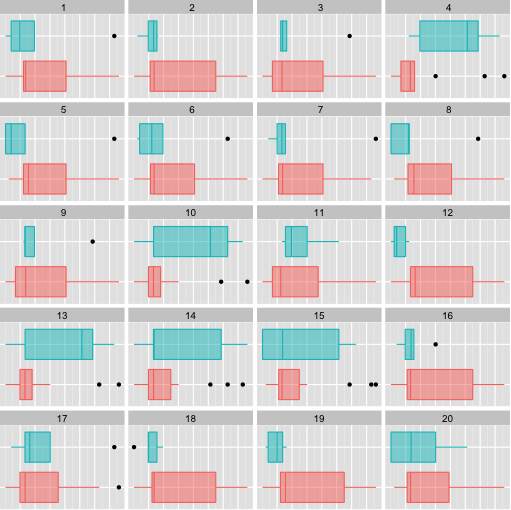
\includegraphics[height=\textwidth]{lineup.png}
          (a) ``Which of these plots is the most different from the others?"
        %
        \end{minipage}
      %  \hfill
        \begin{minipage}[c]{.4\textwidth}
        \centering
          \includegraphics[height=.5\textwidth]{Figure/fig-biplots-pca5-1}\\
          \includegraphics[height=.5\textwidth]{Figure/fig-biplots-pca5-2}\\
        (b) Biplots of visuo-spatial tests and lineup task.
        \end{minipage}
    \caption{\protect\label{fig:lineup}On the left a sample lineup of boxplots is shown. Participants are asked to identify the most different plot.  %Participants are instructed to choose the plot which appears most different from the others. 
    Panel 4 is the target plot, because the two groups have a large difference in medians.
    The biplots on the right show principal components 2-5 with observations from the user study. The lineup task appears to be most similar to the figure classification task.}
  }




%% Uncomment below to disable the manuscript note
%\renewcommand{\manuscriptnotetxt}{}

%% Copyright space is enabled by default as required by guidelines.
%% It is disabled by the 'review' option or via the following command:
% \nocopyrightspace

%%%%%%%%%%%%%%%%%%%%%%%%%%%%%%%%%%%%%%%%%%%%%%%%%%%%%%%%%%%%%%%%
%%%%%%%%%%%%%%%%%%%%%% START OF THE PAPER %%%%%%%%%%%%%%%%%%%%%%
%%%%%%%%%%%%%%%%%%%%%%%%%%%%%%%%%%%%%%%%%%%%%%%%%%%%%%%%%%%%%%%%%
\IfFileExists{upquote.sty}{\usepackage{upquote}}{}
\begin{document}

%% The ``\maketitle'' command must be the first command after the
%% ``\begin{document}'' command. It prepares and prints the title block.

%% the only exception to this rule is the \firstsection command
\firstsection{Introduction}

\maketitle



\label{sec:introduction}Data displays provide quick summaries of data, models, and results, but not all displays are equally good, nor is any data display equally useful to all viewers. 
Graphics utilize higher-bandwidth visual pathways to encode information~\cite{baddeley1974working}, allowing viewers to quickly and intuitively relate multiple dimensions of numerical quantities.
Well-designed graphics emphasize and present important features of the data while minimizing  features of lesser importance, guiding the viewer towards conclusions that are meaningful in context and supported by the data while maximizing the information encoded in working memory. Under this framework, well-designed graphics reduce memory load and make more cognitive resources available for other tasks (such as drawing conclusions from the data), at the cost of depending on certain visuospatial reasoning abilities. 

Many theories of graphical learning center around the difference between visual and verbal processing: the dual-coding theory emphasizes the utility of complementary information in both domains, while the visual argument hypothesis emphasizes that graphics are more efficient tools for providing data with spatial, temporal, or other implicit ordering, because the spatial dimension can be represented graphically in a more natural manner~\cite{vekiri2002value}. Both of these theories suggest spatial ability impacts a viewer's use of graphics, because spatial ability either influences cognitive resource allocation or affects the processing of spatial relationships between graphical elements. In addition, previous investigations into graphical learning and spatial ability have found relationships between spatial ability and the ability to read information from graphs~\cite{lowrie2007solving}. 
However,  mathematical ability, not spatial ability, was shown~\cite{shah1995conceptual} to be associated with accuracy on a simple two-dimensional line graph. 
Spatial ability becomes more important when more complicated graphical displays are used in comparison tasks: the lower performance of individuals with low spatial ability on tests utilizing diagrams and graphs is attributed~\cite{mayer1994whom} to the fact that more cognitive resources are required to process the visual stimuli, which leaves fewer resources to make connections and draw conclusions from those stimuli. It is theorized that graphics are a form of ``external cognition"~\cite{scaife1996external} that guide, constrain, and facilitate cognitive behavior~\cite{zhang1997nature}. 

Here, we want to investigate the extent to which observers make use of spatial ability in their evaluation of and reasoning about statistical graphics. As a quantitative measure of how successful an evaluation is, we are making use of the lineup protocol~\cite{buja2009statistical, wickham2010graphical, majumder2013validation}. 

``Lineups" were introduced as a tool to evaluate the statistical significance of a graphical finding~\cite{wickham2010graphical}. Lineups are also useful in assessing the effectiveness of alternative graphical displays~\cite{hofmann2012graphical, loy:2015}. Like their police counterpart, graphical lineups consist of several distractor plots (of randomly generated data) and one target (the data plot).  Figure~\ref{fig:lineup}(a) shows a sample lineup of boxplots; in this example, sub-plot 4 shows the target data (recognizable by the shift between the two boxplot medians).


%This method is described in more detail in the next section; here we motivate the importance of understanding the connection between lineups and spatial reasoning. 


Lineups provide a quantitative measurement of the effectiveness of a particular plot: if participants consistently identify the target plot rather than the randomly-generated distractors, the plot effectively shows the difference between real data and random noise. 
This removes much of the subjectivity from user evaluations of display effectiveness, and the procedure is simple enough that it does not generally require participants to be very familiar with data-based graphics. 
While previous research~\cite{lowrie2007solving,mayer1994whom} has examined the link between certain types of graphical perception and spatial skills, it is important to identify any additional visual skills participants utilize to complete the lineup task, as well as better understand demographic characteristics (math education, research experience, age, gender) which may impact performance~\cite{humanfactorslineups}. 

In this paper, we present the results of a study designed to compare lineup performance with visual aptitude and reasoning tests, examining the skills necessary to successfully evaluate lineups. 
Our goal in this study is not to evaluate the statistical significance of particular plots or visualization designs, but rather, to consider the cognitive demands that we require of participants in lineup studies. 


We compare lineup performace to the visual search task (VST), paper folding test, card rotation test, and figure classification test. The last three tests are part of the Kit of Factor-Referenced Cognitive Tests~\cite{educational1963kit, ekstrom1976manual}. These tests measure three separate dimensions of visuospatial ability and have been virtually unchanged in use  since the 1960s, and are thus extremely well-studied.  

The VST measures visual search speed~\cite{goldstein1973validity}; we considered visual search as the basis of a lineup evaluation and included this test mainly to identify potential problems in the results, if participants were unable to perform this task. 
Both  card rotation and paper folding tests measure spatial manipulation ability in two- and three dimensions, while the figure classification test measures inductive reasoning~\cite{ekstrom1976manual}; 
we hypothesized that all of these skills are recruited during the lineup task, but are interested which of these dominate in predicting performance on the lineup task. 

We hope to facilitate comparison of the lineup task to known cognitive tests, inform the design of future studies, and better understand the perception of statistical lineups. 

In section \ref{sec:methods} we introduce the tests used in the study and describe how the tests are scored. In section \ref{sec:results} we discuss the study results and compare them with scores on previously established tests, accounting for demographic characteristics associated with test scores. We discuss multi-collinearity in the study results, and use principal components analysis and linear models to draw some conclusions about the similarity between lineups and aptitude tests. Finally, in section \ref{sec:discussion}, we discuss the implications of the study results for the lineup protocol and  possible extensions. 

\paragraph{Related Work}
It has been shown~\cite{pak2014} that visualizations do not necessarily reflect statistical properties well and may even mislead viewers~\cite{correll2013}. Lineup tests approach the evaluation of statistical visualizations differently; they do not ask participants to judge significances or estimate numerical differences directly (as in \cite{cleveland:1985, fuchs, talbot}) but are only based on comparisons. Statistical properties are then derived from this assessment using results aggregated across individual participants.  This has been shown to be similarly powerful to standard statistical tests in situations where these classical tests hold, and more powerful in situations where conditions of classical tests are not met~\cite{majumder2013validation}. The difference between statistical properties and visualizations is very easy to explain, as statistical significance of, e.g. a correlation coefficient is based on only a few summary statistics, whereas e.g. a corresponding scatterplot shows the data in more detail, perhaps leading participants to a different evaluation. This, however, is not a drawback of the visualization but only shows that summary statistics might not be enough to come to an appropriate conclusion \cite{anscombe:1973}. 

\section{Methods}\label{sec:methods}

\subsection{The Lineup Protocol}
The lineup protocol~\cite{hofmann2012graphical,wickham2010graphical, buja2009statistical} is a testing framework that allows researchers to quantify the statistical significance of a graphical finding with the same mathematical rigor as conventional hypothesis tests.

In a lineup test, the plot of the data is placed randomly among a set of, generally 19, distractor plots (or {\it null plots}) that are rendered from data generated by a model, without a signal (a null model). This sheet of charts is then shown to human observers, who are asked to identify the display that is ``the most different" 
This phrasing is intentionally ambiguous to prevent biasing participants and is commonly used in other studies employing lineups~\cite{wickham2010graphical, majumder2013validation}.
If an observer identifies the plot drawn from the actual data, this can be reasonably taken as evidence that the data it shows is different from the data of other plots.
Let $X$ be the number of observers (out of $n$) who identify the data plot from the lineup. Under the null hypothesis that the data plot is not different from the other plots, $X$ has approximately a Binomial distribution~\cite{wickham2010graphical, majumder2013validation}. If $k$ of the observers identify the data plot from the lineup, the probability $P(X \ge k)$ is the $p$-value of the corresponding visual test. 
%
By aggregating responses from different individuals the lineup protocol therefore allows an objective evaluation of a graphical finding. 
Additionally, however, we can aggregate the scores from the same individual on several lineups to objectively assess an individual's performance on the lineup task. 

In this experiment, we are interested in individual skill at evaluating lineups rather than the data displayed in a single lineup, so we will consider an individual's aggregate lineup score, derived as follows:

%For this approach, we derive a score for an individual as follows:

Assume that an observer has evaluated $K$ lineups of size $m$ (consisting of $m-1$ decoy plots and 1 target), and successfully identified the target in $n_c$ of these plots, while missing the target in $n_w$ of them. 
The score for this individual is then given as:
\begin{equation}\label{eq.scoring1}
n_c - n_w/(m-1)
\end{equation}
Note that the sum of answers, $n_c + n_w$, is at most $K$, but may be less, if an observer chooses to not answer one of the lineup tasks or runs out of time. The scoring scheme as given in (\ref{eq.scoring1}) is chosen so that if participants are guessing, the expected score is 0. 

Statistical lineups depend on the ability to search for a signal amid a set of distractors (visual search) and the ability to infer patterns from stimuli (pattern recognition). Depending on the choice of plot shown in the lineup, the task of identifying the most different plot might require additional abilities from participants, e.g.~polar coordinates depend on the ability to mentally rotate stimuli (spatial rotation) and mentally manipulate graphs (spatial rotation and manipulation). By breaking the lineup task down into its components, we  determine which visuospatial factors most strongly correlate with lineup performance, using carefully chosen, externally validated, cognitive tests to assess these aspects of visuospatial ability. 

Demographic factors are known to impact lineup performance: country, education, and age affected score on lineup tests, and all of those factors as well as gender had an effect on the amount of time spent on lineups~\cite{humanfactorslineups}. In addition, lineup performance can be partially explained using statistical distance metrics~\cite{distancemetriclineups}, but these metrics do not completely succeed in predicting human performance, in part due to the difficulty of representing human visual ability algorithmically.

One of the most useful features of the lineup protocol is that it allows researchers to determine which visualizations show certain features more conclusively by providing an experimental protocol for comparing different visualization methods based on the accuracy of user conclusions. In addition, lineups provide researchers with a rigorous framework for determining whether a specific graph shows a real, statistically significant effect by comparing a target plot with plots formed using permutations of the same data, providing a randomization test protocol for graphics. As a result, lineups are a useful and innovative tool for evaluating charts; on an individual level, they can also be used to evaluate a specific participant's perceptual reasoning ability in the context of statistical graphics.
This study uses the lineup protocol to examine differences in individual performance, rather than using aggregate scores to determine the effectiveness of a single visualization. 


In this study, we utilize three blocks of statistical lineups; each of these blocks consists of 5-7 datasets, that are displayed in three or four types of plots (examples of the visualization types presented in each block of lineups are shown in figure \ref{fig:lineups}). For example, in the lineups of set 1, the same five datasets are displayed as a dot plot, density plot, box plot, and histogram. Each block of lineups are a subset of stimuli used in experiments designed to compare the visual significance of different plot types, however, our purpose in this study is not to determine the efficacy of different types of plots. Rather, our goal is to compare the cognitive demands required to successfully evaluate these lineups, which display variance difference, mean difference, or violations of normality using common statistical plots.

<<<<<<< HEAD
Each of the three sets of 20 lineups was taken from previous experiments \cite{loy:2015, roy2011visual} examining which type of plot most effectively conveyed important characteristics of the underlying data set. %\hhnote{citations?}
=======
Each of the three sets of 20 lineups was taken from previous experiments examining which type of plot most effectively conveyed important characteristics of the underlying data set. 
>>>>>>> last changes from my side
\begin{figure*}[htbp]\centering
\subfloat[Set 1: Boxplot]{
  \includegraphics[keepaspectratio=T,width=.245\linewidth]{../../Images/Lineups1/boxplot_1_15_5_4_13}}
\subfloat[Set 1: Density plot]{
  \includegraphics[keepaspectratio=T,width=.245\linewidth]{../../Images/Lineups1/density_1_15_5_4_13}}
\subfloat[Set 1: Dotplot ]{
  \includegraphics[keepaspectratio=T,width=.245\linewidth]{../../Images/Lineups1/dotplot_1_15_5_4_13}}
\subfloat[Set 1: Histogram]{
  \includegraphics[keepaspectratio=T,width=.245\linewidth]{../../Images/Lineups1/histogram_1_15_5_4_13}}\\
\subfloat[Set 2: Boxplot]{
  \includegraphics[keepaspectratio=T,width=.245\linewidth]{../../Images/Lineups2/file147f94f6965d7}}
\subfloat[Set 2: Boxplot with jittered points]{
  \includegraphics[keepaspectratio=T,width=.245\linewidth]{../../Images/Lineups2/file147f9e65f0e4}}
\subfloat[Set 2: Bee swarm boxplot]{
  \includegraphics[keepaspectratio=T,width=.245\linewidth]{../../Images/Lineups2/file147f9fc58d73}}
\subfloat[Set 2: Violin plot]{
  \includegraphics[keepaspectratio=T,width=.245\linewidth]{../../Images/Lineups2/file147f93acbb7e4}}\\
\subfloat[Set 3: QQ-plot with guide line]{
  \includegraphics[keepaspectratio=T,width=.245\linewidth]{../../Images/Lineups3/file13876a225d34-single}}
\subfloat[Set 3: QQ-plot with acceptance bands]{
  \includegraphics[keepaspectratio=T,width=.245\linewidth]{../../Images/Lineups3/file13877c93dc78-single}}
\subfloat[Set 3: QQ-plot rotated 45 degrees.]{
  \includegraphics[keepaspectratio=T,width=.245\linewidth]{../../Images/Lineups3/file13878e5c92f-single}}
\protect\caption{Lineup plot types used in the experiment. \label{fig:lineups} Each set of plots is representative of the plot types shown in a block of lineups in the experiment, and each block represents a subset of plots from a traditional lineup experiment to determine which visualization method facilitates identification of the plot with the strongest visual signal. Set 1 manipulates group means and variance, set 2 manipulates group means, and set 3 examines violations of normality. These tasks were chosen as common statistical visualization tasks, and while not exhaustive, should provide a broad basis for interpreting the results of this experiment.}
\end{figure*}



\begin{table*}[htbp]\centering
\begin{tabular}{rlllc}
\hline
  & Card Rotation & Paper Folding & Figure Classification & Visual Search  \\\hline
ISU Students & 83.4 (24.1) 
             & 12.4 (3.7)
             & 57.0 (23.8)\footnotemark[1]
             & 21.9 (2.3)\\
Scaled Scores & 88.0 (34.8)
              & 13.8 (4.5)
              & 58.7 (14.4)\footnotemark[2]
              & -- \\
Unscaled Scores & 44.0 (24.6)\footnotemark[3]
                & 13.8 (4.5)
                & \parbox[c]{.2\linewidth}{M:~120.0~(30.0)\\ F:~114.9~(27.8)}
                & --\\\hline
{\footnotesize Population}    
              & \parbox[t]{.15\linewidth}{\footnotesize approx.\ 550 male\\ naval recruits} 
              & \parbox[t]{.17\linewidth}{\footnotesize 46 college students\\(1963~version)}
              & \parbox[t]{.2\linewidth}{\footnotesize suburban 11th \& 12th \\ grade students\\(288-300 M, 317-329 F)}
              & \\\hline
\end{tabular}
\caption[Comparison of scores for cognitive tasks.]{Comparison of scores from Iowa State students and scores reported in~\protect~\cite{ekstrom1976manual}. Scaled scores are calculated based on information reported in the manual, scaled to account for differences in the number of questions answered during this experiment. Data shown are from the population most similar to ISU students, out of the data available. The visual search task~\protect~\cite{goldstein1973validity,demita1981validity,moerland1986neuropsychological} is not part of the Kit of Factor Referenced Cognitive Test data, and thus we do not have comparison data for the form used in this experiment.
\label{tab:scorecomparison}}
\end{table*}

\paragraph{Lineup Set 1}
The lineups in this set are taken from an experiment which examined the use of boxplots, density plots, histograms, and dotplots to compare two groups which vary in mean and sample size. This set of lineups consists of 20 plots selected from the plots used in the full experiment; each set of data is displayed with each of the four plot types. Figure \ref{fig:lineups} (a)-(d) provides an example of the four plot types displaying the same data.\hphantom{\ref{tab:scorecomparison}}


\paragraph{Lineup Set 2}
The lineups in the second set are taken from another experiment which examined visualizations of categorical data, this time comparing boxplots, bee swarm boxplots, boxplots with overlaid jittered data, and violin plots, as shown in figure \ref{fig:lineups} (e)-(h). Participants were much more accurate in this experiment than in the experiment described previously, because of the types of plots compared as well as the underlying data distributions. 

\paragraph{Lineup Set 3}
Lineups in the final set are taken from an experiment which examined modifications of QQ-plots, using data from various model simulations. Reference lines, acceptance bands, and rotation were utilized to examine which plots allowed participants to most effectively identify violations of normality. Rotated QQ-plots showed lower performance because participants were able to more accurately compare acceptance bands to residuals, and thus could identify that the reference bands were overly liberal. As a result, performance was somewhat lower for rotated plots, even though participants were more accurate when comparing the residuals to the reference bands \cite{loy:2015}.

\subsection{Measures of visuospatial ability}

Participants are asked to complete several cognitive tests designed to measure spatial and reasoning ability. Tasks are timed such  that participants are under pressure; participants are not expected to finish all of the problems in each section. This allows for better discrimination between scores and reduces score compression at the top of the range. 

The \textbf{visual searching task} (VST), shown in figure~\ref{fig:VST}, is designed to test a participant's ability to find a target stimulus in a field of distractors, thus making the visual search task similar in concept to lineups. Historically, this visual search task has been used as a measure of brain damage~\cite{goldstein1973validity,demita1981validity,moerland1986neuropsychological}; however, similar tasks have been used to measure cognitive performance in a variety of situations, for example under the influence of drugs in~~\cite{anderson1983interactive}. The similarity to the lineup protocol as well as the simplicity of the test and its' lack of color justify the slight deviation from forms of visual search tasks typically used in normal populations, such as those in~\cite{wolfe1990limitations,treisman1980feature}. 
We have included visual search in the cognitive testing battery for this experiment because it is the most simple of the tasks required to successfully evaluate a lineup; if participants cannot complete visual search tasks successfully, they will not be able to accurately identify which lineup plot is different. 


\begin{figure}[htp]\centering
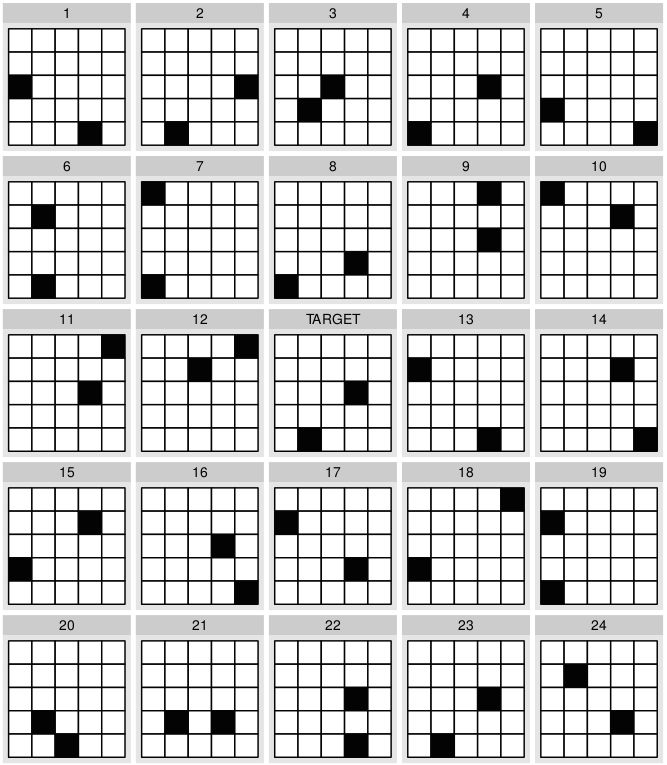
\includegraphics[width=.8\linewidth]{VisualSearch}
\caption[Visual Search Task]{Visual Search Task (VST). Participants are instructed to find the plot numbered 1-24 which matches the plot labeled ``Target". Participants will complete up to 25 of these tasks in 5 minutes.}\label{fig:VST}
\end{figure}

The remaining cognitive tests are adapted from \cite{ekstrom1976manual} and are highly validated tests that have been constructed to measure specific cognitive factors, such as inductive reasoning and spatial rotation.

The \textbf{figure classification task} tests a participant's ability to extrapolate rules from provided figures. This task is associated with inductive reasoning abilities (factor I  in~\cite{ekstrom1976manual}). An example is shown in figure~\ref{fig:figureclassification}. 

The figure classification test requires the same type of reasoning as the lineups: participants must determine the rules from the provided classes, and extrapolate from those rules to classify new figures. In lineups, participants must determine the rules based on the panels appearing in the lineup; they must then identify the plot which does not conform. As such, the figure classification test has content validity in relation to lineup performance: it is measuring similar underlying criteria. 

The \textbf{card rotation test} measures a participant's ability to rotate objects in two dimensions in order to distinguish between left-hand and right-hand versions of the same figure. It tests mental rotation skills, and is classified as a test of spatial orientation in~\cite{ekstrom1976manual}, though it does require that participants have both mental rotation ability and short-term visual memory. An example is shown in figure~\ref{fig:cardrotation}. 
The card rotation test is often used in studies investigating the effect of visual ability on the use of visual aids~\cite{mayer1994whom} and statistical graphs~\cite{lowrie2007solving} in education.

Two-dimensional comparisons are an important component of lineup performance. In some lineup situations, these comparisons sometimes involve translation, but in other lineups, rotation is required. Lineups also require visual short-term memory, so the additional factor measured implicitly by this test does not reduce its potential relevance to lineup performance. 
Three-dimensional rotation is somewhat less relevant to most statistical graphics, which are typically two-dimensional in nature. While \cite{ekstrom1976manual} includes three-dimensional rotation tasks similar to \cite{shepard1971mental}, these three-dimensional tasks were not included in this experiment due to time constraints and limited face validity.

The \textbf{paper folding test} measures participants' ability to visualize and mentally manipulate figures in three dimensions. A sample question from the test is shown in figure~\ref{fig:paperfolding}. It is classified as part of the visualization factor in~\cite{ekstrom1976manual}, which differs from the spatial orientation factor because it requires participants to visualize, manipulate, and transform the figure~mentally, which makes it a more complex and demanding task than simple rotation. The paper folding test is associated with the ability to extrapolate symmetry and reflection.

Tests in the Kit of Factor-Referenced Cognitive tests are classified according to the reasoning required to complete the test; in this way, we can be reasonably sure that the paper folding test, card rotation test, and figure classification test have construct validity.

\begin{figure}[ht]
  \centering
   \subfloat[Figure Classification Task. Participants classify each figure in the second row as belonging to one of the groups above. Participants complete up to 14 of these tasks (each consisting of 8 figures to classify) in 8 minutes.\label{fig:figureclassification}]{%
  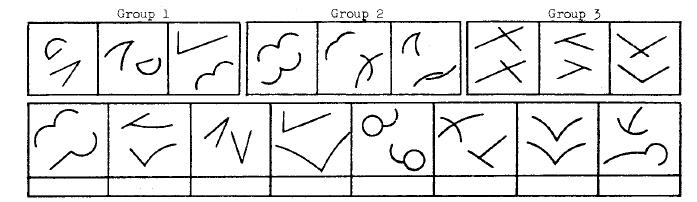
\includegraphics[width=.8\linewidth]{figureclassification}
}
\hfill
    \subfloat[Card Rotation Task. Participants mark each figure on the right hand side as either the same as or different than the figure on the left hand side of the dividing line. Participants complete up to 20 of these tasks (each consisting of 8 figures) in 6 minutes.\label{fig:cardrotation}]{%

\includegraphics[width=.8\linewidth]{cardrotation}
    }
    \hfill
    \subfloat[Paper Folding Task. Participants are instructed to pick the figure matching the sequence of steps shown on the left-hand side. Participants  complete up to 20 of these tasks in 6 minutes.\label{fig:paperfolding}]{%
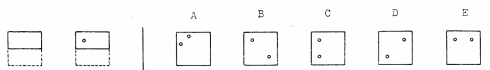
\includegraphics[width=.8\linewidth]{paperfolding}
   }
    \caption{Visuospatial tests}
    \label{fig:tests}
\end{figure}

Lineups require similar manipulations in two-dimensional space, and also require the ability to perform complex spatial manipulations mentally; for instance, comparing the interquartile range of two boxplots as well as their relative alignment to a similar set of two boxplots in another panel.

\paragraph{Experimental Procedure}
All tasks (cognitive and lineups) were provided to participants on paper \newtext{in a supervised lab setting}, to conform to the procedure used in~\cite{ekstrom1976manual}. The order of tasks was the same for each participant due to the constraints of in-person testing; an internal pilot study did not indicate an effect of task order, \newtext{nor did the pilot results suggest an interaction/learning effect from one task to the next.}


Between cognitive tasks, participants were asked to complete three blocks of 20 lineups each, assembled from previous studies~\cite{hofmann2012graphical,majumder2013validation}. Participants were given 5 minutes to complete each block of 20 lineups. Figure~\ref{fig:lineup}(a) shows a sample lineup of box plots. 

In addition to these tests, participants completed a questionnaire on personal background and demographics, including questions about colorblindness, mathematical training, self-perceived verbal/mathematical/artistic skills, time spent playing video games, and undergraduate major. These questions are designed to assess different factors which may influence a participant's skill at reading graphs and performing spatial tasks. 

After each test or block of lineups, participants were given 1-2 minutes to rest and recover; the order of tests was designed to prevent fatigue on a single task \newtext{(which led us to interweave lineup evaluations)}. The duration of testing for each participant was approximately 1 hour. \newtext{None of the participants who showed up for their scheduled session asked to leave early.} A complete set of test documents (with copyrighted material redacted) is available as supplemental materials. 


\subsection{Test Scoring}\label{sec:scaling}
%
All test results were scored so that random guessing produces an expected value of 0; therefore each question answered correctly contributes to the score by 1, while a wrong answer is scored by $-1/(k-1)$, where $k$ is the total number of possible answers to the question. Thus, for a test consisting of multiple choice questions with $k$ suggested answers with a single correct answer each, the score is calculated as
\begin{eqnarray}\label{eq.scoring}
\# \text{correct answers } - 1/(k-1) \cdot \# \text{wrong answers}
\end{eqnarray}
Equation \ref{eq.scoring} is a restatement of equation \ref{eq.scoring1} provided for convenience.
This allows us to compare each participant's score in light of how many problems were attempted as well as the number of correct responses. Combining accuracy and speed into a single number does not only make a comparison of test scores easier,  this scoring mechanism is also used on many standardized tests, such as the SAT and the battery of psychological tests~\cite{diamond1973correction, ekstrom1976manual} from which parts of this test are drawn. The advantage of using tests from the Kit of Factor Referenced Cognitive tests~\cite{ekstrom1976manual} is that the tests are extremely well studied (including an extensive meta-analysis in~\cite{voyer1995magnitude} of the spatial tests we are using in this study) and comparison data are available from the validation of these factors~\cite{schaie1998longitudinal,hampson1990variations,mayer1994whom} and previous versions of the kit~\cite{educational1963kit}.


\section{Results}\label{sec:results}
Results are based on an evaluation of 38 undergraduate students at Iowa State University. 61\% of the participants were in STEM fields, the others were distributed relatively evenly between agriculture, business, and the social sciences. Students were evenly distributed by gender, and were between 18 and 24 years of age with only one exception in the 25-28 bracket. This is reasonably representative\footnote{\url{http://www.registrar.iastate.edu/sites/default/files/uploads/stats/university/F14summary.pdf}} of the student population of Iowa State; in the fall 2014 semester, 26\% of students were associated with the college of engineering, 24\% were associated with the college of liberal arts and sciences, 15\% were associated with the college of human sciences, 7\% with the college of design, 13\% with the business school, and 15\% with the school of agriculture.  

\subsection{Comparison of Spatial Tests with Validated Results}
The card rotation, paper folding, and figure classification tests have been validated using different populations, many of which are demographically similar to Iowa State students (naval recruits, college students, late high-school students, and 9th grade students). We compare Iowa State students' unscaled scores in Table~\ref{tab:scorecomparison}, adjusting data from other populations to account for subpopulation structure and test length. 

Table~\ref{tab:scorecomparison} shows mean scores and standard deviation for ISU students and other populations. Values have been adjusted to accommodate for differences in test procedures and sub-population structure; for instance,  some data is reported for a single part of a two-part test, or results are reported for each gender separately (adjustment procedure is described in more detail in Appendix~\ref{app:ScoreAdj}). Once adjusted, it is evident that Iowa State undergraduates scored at about the same level as other similar demographics. In fact, both means and standard deviations of ISU students' scores are similar to the comparison groups, which were chosen from available demographic groups based on population similarity. 

Comparison population data was chosen to most closely match ISU undergraduate population demographics. Thus, if comparison data was available for 9th and 12th grade students, scores of Iowa State students were compared to scores of 12th grade students, who are closer in age to college students. When data was available from college students and Army enlistees, comparisons of scores were based on other college students, as college students are more likely to have a similar gender distribution to ISU students.

Applying the grading protocol discussed in section~\ref{sec:scaling}, we see that the ranges of lineup and visuospatial test scores do not include zero; this indicates that we do not see random guessing from participants in any task. Figure~\ref{fig:Scores} shows the range of possible scores and the observed score distribution. 
Participants' scores on the VST indicate score compression; that is, both participants with medium and high visual search abilities scored at the extremely high end of the spectrum. 
In future experiments, participants should be given less time (or more questions) to better differentiate participants with medium and high-ability.


\begin{figure}[ht]
\centering
\includegraphics[width=.9\linewidth]{Figure/fig-ResultsScaledScores-1}
\caption{Test scores for lineups and visuospatial tests. As none of the participants scored at or below zero, we can conclude that there is little evidence of random guessing. We also note the score compression that occurs on the Visual Search test; this indicates that most participants scored extremely high, and thus, participants' scores are not entirely representative of their ability. \label{fig:Scores}}
\end{figure}
% 
%\afterpage{\clearpage}

% Applying the grading protocol discussed in section~\ref{sec:scaling}, we see that the ranges of lineup and visuospatial test scores do not include zero; this indicates that we do not see random guessing from participants in any task. Figure~\ref{fig:Scores} shows the range of possible scores and the observed score distribution. 


\subsection{Lineup Performance and Demographic Characteristics}


\begin{figure}[h!tb]\centering
\includegraphics[width=.95\linewidth]{fig-VisReasoningCategorical-1}
\caption[Visual Aptitude Study Results]{Demographic characteristics of participants compared with lineup score. Categories are ordered by effect size; majoring in a STEM field, calculus completion, hours spent playing video games per week, and sex are all associated with a significant difference in lineup score. }\label{fig:visualaptitudecat}
\end{figure}
%\afterpage{\clearpage}

%Next, we examine the effect of demographic factors on lineup performance. 
Previous work found a relationship between lineup performance and demographic factors such as education level, country of origin, and age~\cite{humanfactorslineups}; our participant population is very homogeneous, which allows us to explore factors such as educational background and skills on performance in lineup tests. 

Figure~\ref{fig:visualaptitudecat} shows participants' lineup scores in relationship to their responses in the questionnaire given at the beginning of the study; this allows us to explore effects of demographic characteristics (major, research experience, etc.) on test performance. 

Completion of Calculus I is associated with increased performance on lineups; this may be related to general math education level, or it may be that success in both lineups and calculus requires certain visual skills. This association is consistent with findings in~\cite{shah1995conceptual}, which associated  mathematical ability to performance on simple graph description tasks.  There is also a significant relationship between hours of video games played per week and score on lineups, however, this association is not monotonic and the groups do not have equal sample size, so the conclusion may be suspect. There is a (nearly) significant difference between male and female performance on lineups; this is not particularly surprising, as men perform better on many spatial tests~\cite{voyer1995magnitude} and performance on spatial tests is correlated with phase of the menstrual cycle in women~\cite{hausmann2000sex}. There is no significant difference in lineup performance for participants of different age, self-assessed skills in various domains, previous participation in math or science research, completion of a statistics class, or experience with AutoCAD. These demographic characteristics were chosen to account for life experience and personal skills which may have influenced the results. Statistical test results are available in Appendix~\ref{app:categoricalresults}. 

\subsection{Visual Abilities and Lineup Performance}



\begin{figure}[ht]
\centering
\includegraphics[width=.9\linewidth]{Figure/fig-VisReasoningSPM-1}
\caption{Pairwise scatterplots of test scores. Lineup scores are most highly correlated with figure classification scores, and are also highly correlated with card rotation scores. Paper folding and card rotation scores are also highly correlated.\label{fig:scatterplotmatrix}}
\end{figure}
%\afterpage{\clearpage}



Results from the visuospatial tests used in this experiment are highly correlated, as shown in Figure~\ref{fig:scatterplotmatrix}; this is to be expected given that all of these tests are in some way measuring individuals' visual ability. 
While test scores are correlated, the relationships between test scores appear to be linear, with sufficient variability around the trend line to merit further investigation. The correlations are to be expected, as all of the tests in this experiment are conducted in a visual domain, and require general reasoning, intelligence, and other factors. 
What is of more interest to us is whether lineups recruit specific cognitive abilities, such as visual search, reasoning and categorization ability, mental rotation.
In order to assess factors contributing to lineup performance, we first examine the separate dimensions measured by the battery of cognitive tests (other than lineups) using principal components analysis on the scaled test scores, then we examine all five tests (four cognitive tests, and additionally lineups) using the same procedure. 

Principal component analysis (PCA) is a statistical technique to transform the coordinate system of correlated data, producing orthogonal components in a new coordinate space (see~\cite{pcaReference} for more information). The most stringent assumption required for PCA is that of linearity, which is reasonable given Figure \ref{fig:scatterplotmatrix}. Additionally, PCA assumes that the interesting portion of the data is the variance between any two variables (a perfectly linear relationship between two variables would be uninteresting, as the variables contain the same information). As a result, PCA can be used to examine which variables contain similar information (i.e. which variables are represented in each principal component). It is this feature of principal components which we utilize in this paper. 

A principal component analysis of the four established visuo-spatial tests reveals that they all share a very strong first component, which explains about 64\% of the total variability. Principal components (PC-) are ordered by importance (how much variability in the data they contain), and each principal component is uncorrelated with every other principal component. 

PC1 is essentially an average across all tests representing a general ``visual intelligence" factor. The other principal components span another two dimensions, while the last dimension is weak (at 6\%). 
PC2 differentiates the figure classification test from the visual searching test, whereas PC3 differentiates these two tests from the paper folding test. 
% More detailed results from the 4-test analysis are provided in Appendix~\ref{app:pca}.

% latex table generated in R 3.1.1 by xtable 1.7-3 package
% Sat Jun 27 22:50:13 2015
\begin{table}[htb]
\centering
\caption{Importance of principal components in an analysis of four tests of spatial ability: figure classification, paper folding, card rotation, and visual search.\label{tab:PCAvariance4}} 
{\footnotesize
\begin{tabular}{rrrrr}
  \hline
 & PC1 & PC2 & PC3 & PC4 \\ 
  \hline
Standard deviation & 1.61 & 0.81 & 0.73 & 0.49 \\ 
  Proportion of Variance & 0.64 & 0.16 & 0.13 & 0.06 \\ 
  Cumulative Proportion & 0.64 & 0.81 & 0.94 & 1.00 \\ 
   \hline
\end{tabular}
}
\end{table}

Table~\ref{tab:PCAvariance4} contains the proportion of the variance in the four cognitive tasks represented by each principal component. PC1 accounts for about 60\% of the variance; Figure~\ref{fig:biplots4} and Table~\ref{tab:PCArotation4} confirm that PC1 is a measure of the similarity between all 4 tests; that is, a participant's general (or visual) aptitude. PC2 differentiates the figure classification test from the visual searching test, while PC3 differentiates these two from the paper folding test. PC4 is not particularly significant (it accounts for 5.9\% of the variance), but it differentiates the card rotation task from the paper folding task.

% latex table generated in R 3.1.1 by xtable 1.7-3 package
% Sat Jun 27 22:50:13 2015
\begin{table}[htb]
\centering
\caption{Rotation matrix for principal component analysis of the four cognitive tests (visual search, paper folding, card rotation, figure classification).\label{tab:PCArotation4}} 
{\footnotesize
\begin{tabular}{rrrrr}
  \hline
 & PC1 & PC2 & PC3 & PC4 \\ 
  \hline
Card Rot & 0.55 & -0.19 & -0.38 & 0.72 \\ 
  Fig Class & 0.46 & 0.58 & 0.66 & 0.14 \\ 
  Folding & 0.52 & 0.33 & -0.53 & -0.59 \\ 
  VST & 0.46 & -0.72 & 0.38 & -0.34 \\ 
   \hline
\end{tabular}
}
\end{table}


\begin{knitrout}
\definecolor{shadecolor}{rgb}{0.969, 0.969, 0.969}\color{fgcolor}\begin{figure}

{\centering \includegraphics[width=.45\linewidth]{Figure/fig-biplot-pca4-1} 
\includegraphics[width=.45\linewidth]{Figure/fig-biplot-pca4-2} 

}

\caption{Biplots of principal components 1-4 with observations (same as figure 1(b)). Principal component analysis was performed on the four cognitive tests used to understand the association between the cognitive skills required for these tests and the skills required for the lineup protocol.  \label{fig:biplots4}}\label{fig:biplot-pca4}
\end{figure}


\end{knitrout}
Figure~\ref{fig:biplots4} shows that the first PC does not differentiate between any of the tasks; it might be best understood as a general aptitude factor. All of the remaining principal components distinguish between the cognitive tasks; we can utilize this separation by incorporating the lineup task and examining changes in the principal components. 

Next, we add the lineup results to our principal components analysis. The results of the principal component analysis of the four cognitive tests and lineup results are similar to the results of the cognitive tests alone; this suggests that lineups require at least some of the skills measured by the other cognitive tests. Table~\ref{tab:PCAvariance5} shows the importance of each principal component; from the distribution of the variance components, we see that the lineup test spans an additional dimension within the space of the four established tests. 
% latex table generated in R 3.1.1 by xtable 1.7-3 package
% Sat Jun 27 22:50:13 2015
\begin{table}[ht]
\centering
\caption{Importance of principal components, analyzing all five tests.\label{tab:PCAvariance5}} 
{\footnotesize
\begin{tabular}{rrrrrr}
  \hline
 & PC1 & PC2 & PC3 & PC4 & PC5 \\ 
  \hline
Standard deviation & 1.73 & 0.84 & 0.75 & 0.70 & 0.48 \\ 
  Proportion of Variance & 0.60 & 0.14 & 0.11 & 0.10 & 0.05 \\ 
  Cumulative Proportion & 0.60 & 0.74 & 0.85 & 0.95 & 1.00 \\ 
   \hline
\end{tabular}
}
\end{table}


% latex table generated in R 3.1.1 by xtable 1.7-3 package
% Sat Jun 27 22:50:13 2015
\begin{table}[ht]
\centering
\caption{PCA Rotation matrix for all five tests. The first principal component is essentially an average of performance on all five tests. \label{tab:PCArotation5}} 
\begin{tabular}{rrrrrr}
  \hline
 & PC1 & PC2 & PC3 & PC4 & PC5 \\ 
  \hline
Lineup & 0.42 & 0.49 & -0.46 & 0.60 & -0.10 \\ 
  Card Rot & 0.50 & -0.30 & 0.28 & 0.23 & 0.73 \\ 
  Fig Class & 0.43 & 0.45 & -0.15 & -0.75 & 0.18 \\ 
  Folding & 0.47 & 0.07 & 0.68 & 0.04 & -0.56 \\ 
  VST & 0.41 & -0.69 & -0.48 & -0.15 & -0.33 \\ 
   \hline
\end{tabular}
\end{table}

From the rotation matrix (see Table~\ref{tab:PCArotation5}) we see that  
the first principal component, PC1, is again essentially an average across all tests and accounts for 60.1\% of the variance in the data. 


\begin{knitrout}
\definecolor{shadecolor}{rgb}{0.969, 0.969, 0.969}\color{fgcolor}\begin{figure}

{\centering \includegraphics[width=.45\linewidth]{Figure/fig-biplots-pca5-1} 
\includegraphics[width=.45\linewidth]{Figure/fig-biplots-pca5-2} 

}

\caption{Biplots of principal components 2-5 with observations. The lineup task appears to be most similar to the figure classification task, based on the plot of PC2 vs. PC3. (These are the same biplots as shown in figure \ref{fig:lineup}b)  \label{fig:biplots5}}\label{fig:biplots-pca5}
\end{figure}


\end{knitrout}
Biplots~\cite{biplots:gabriel} of the remaining components are provided in figure~\ref{fig:biplots5}. Figure classification is strongly related to lineups (PC2, PC3). Performance on the visual search task  is also related to lineup performance (PC3). These two components highlight the shared demands of the lineup task and the figure classification task: participants must establish categories from provided stimuli and then classify the stimuli accordingly. 

The visual search task is also clearly important to lineup performance: PC3 captures the similarity between the visual search and lineup performance, and aspects of these tasks are negatively correlated with aspects of the paper folding and card rotation tasks within PC3. Paper folding does not seem to be strongly associated with lineup performance outside of the first principal component; card rotation is only positively associated with lineup performance in PC4.

PC4 captures the similarity between lineups and the card rotation task and separates this similarity from the figure classification task; this similarity does not account for much extra variance (10\%), but it may be that only some lineups require spatial rotation skills. PC5 contains only 5\% of the remaining variance, and is thus not of much interest, however, it seems to capture the relationship between the card rotation task and the paper folding and visual search tasks.

Figure classification is strongly related to lineups, and as in the four-component PCA, figure classification is strongly represented in the first two principal components. While lineups do span a separate dimension, the PCA suggests that they are most closely related to the figure classification task, and least related to the visual searching task.

This emphasizes the underpinnings of lineups: the test utilizes a visual medium, but ultimately lineups are a classification task presented in a graphical manner. Using lineups as a proxy for statistical significance tests is similar to using a classifier on pictoral data: while the data is presented ``graphically", the participant is actually classifying the data based on underlying summary statistics.

\subsection{Linear model of demographic factors}
Note that many of the demographic variables in the survey show dependencies, for example there is a high correlation between STEM majors and taking calculus. Similarly, the correlation  between having taken a statistics class and having been involved in mathematics or statistics research is high. Only one student is doing research who has not taken a statistics course. Students' ratings of their math skills are also related to whether they are majoring in a STEM field or whether they have completed calculus.

A principal component of the five math/stats questions splits the variables into two main areas: the first principal component is an average of math skills, calculus 1 and STEM, while the second principal component is an average of having taken a statistics class and doing research. We therefore decided to use sums of these variables to come up with a separate math and a stats score. Note, that the correlation between the math and the stats score is almost zero. 

We fit a linear model of lineup scores in the thus modified demographic variables and the test scores from the visuo-spatial tests, selecting the best model using AIC and stepwise backwards selection. The result is shown in Table~\ref{tab:m1}. Only two covariates stay in the model: PC1 and MATH, reflecting two dimensions of what affects lineup scores. We can think of PC1 as a measure of innate visual or intellectual ability, while the MATH score is a matter of both ability and training. The remaining principal components were not sufficiently associated with lineup score to be included in the model.

% latex table generated in R 3.1.1 by xtable 1.7-3 package
% Sat Jun 27 22:50:14 2015
\begin{table}[ht]
\centering
\caption{Estimates and significances of a linear model of lineup scores.} 
\label{tab:m1}
\begin{tabular}{rrrrr}
  \hline
 & Estimate & Std. Error & t value & Pr($>$$|$t$|$) \\ 
  \hline
(Intercept) & 14.1192 & 1.9149 & 7.37 & 0.0000 \\ 
  PC1 & 1.7672 & 0.5230 & 3.38 & 0.0018 \\ 
  MATH & 2.1246 & 0.8732 & 2.43 & 0.0202 \\ 
   \hline
\end{tabular}
\end{table}

%\afterpage{\clearpage}
%
\subsection{Visual Aptitude for Specific Lineup Tasks}
Figure~\ref{fig:lineuptaskmatrix} shows the correlations between the three lineup tasks and the figure classification, card rotation, and paper folding tasks. 
%The visual search task is only slightly correlated with the three lineup tasks and is therefore omitted from this figure.

Performance on lineup tasks 1 and 2, which dealt with the distributuion of two groups of numerical data, is most strongly correlated with the performance on the figure classification task, which measures general reasoning ability.
Performance on lineup task 3, which investigated the potential to visually identify nonnormality in residual QQ-plots, is more associated with the card rotation and paper folding tests, which measure visuospatial ability. This suggests that certain lineup tasks may require more visual ability than others; in the case of the QQ-lineups a successful evaluation  needed  participants to mentally rotate plots to compare vertical distances, requiring more mental manipulation than the first two lineup tasks, which asked from participants to examine categorical data.




\begin{figure}[ht]
\centering
\includegraphics[width=\linewidth]{Figure/fig-LineupTypeSPM-1}
\caption{Pairwise scatterplots of test scores, with lineups separated into the three lineup tasks. All lineup tasks are moderately correlated with the figure classification task, and while tasks 1 and 2 are most strongly correlated with figure classification, lineup task 3 is most strongly correlated with the card rotation and paper folding tasks. \label{fig:lineuptaskmatrix} While the correlations shown in this graph are all less than 0.60, there are some surprisingly strong relationships for human subjects data.}
\end{figure}


In order to examine which lineup tasks are most closely associated with visual abilities tested in the aptitude portions of an experiment, we employ principal component analysis on participant scores averaged across each block of lineups.

Principal component analysis separates multivariate data into orthogonal components using a rotation matrix to transform correlated input data into an orthogonal space. The importance of a principal component is also evaluated to assess the proportion of the overall variance in the data contained within the component (Table \ref{tab:PCAvariance5} shows the importance of each PC for the analysis of the aggregate lineup score and the four aptitude tests). 


\begin{figure}[ht]
\includegraphics[width=\linewidth]{Figure/fig-lineupblockpca-1}
\caption{Principal Component influence plot, showing each input variable's contribution to the principal component, scaled by the proportion of variability in the data contained in the principal component.\label{fig:influence}}
\end{figure}

For variables $X_i$, $i=1, ..., K$ a principal component analysis results in a set of $K$ principal  components $PC_j$, $j=1, ..., K$, given as the rows of the rotation matrix, $M$ (which has dimension $K\times K$, indexed by $i$ and $j$ respectively).
The importance $I_j$ of each component is determined by the amount of variability the data exhibits along each of the principal axis.
The influence of variable $X_i$ on component $PC_j$ is then defined as:
%
$$\text{Influence of variable } X_i \text{ on PC}_j = M_{ij}\times I_j$$
%
Influence is therefore a measure of the contribution of an input variable to the principal component, scaled by the importance of that principal component to the overall variability in the data. Small (absolute) values indicate that there is little influence of $X_i$ on $PC_j$; negative values show the direction of the influence (to maintain the separation of variables as part of principal components analysis). 

Figure~\ref{fig:influence} shows the influence of each input variable on each principal component for a principal component analysis  including each lineup task as a separate input variable. The input variables are shown on the $y$ axis, with the influence of the variable on each PC shown on the $x$ axis. This allows us to consider the rotation matrix visually (while accounting for the importance of each principal component); for instance, we see that again, the first PC accounts for most of the variance and seems to represent general visual aptitude. 

PC2 emphasizes the overlapping variation in performance on lineup test 1 and the figure classification test. PC3 emphasizes the additional variation in performance on lineup test 3 and the visual search test, while PC4 emphasizes the extra variability in performance on lineup test 2 and the paper folding test. All three lineups, plus the figure classification, paper folding, and visual search tests contribute to PC5. PC6 and PC7 jointly account for less than 10\% of the variance in the data and do not display any distinct patterns in the loadings. 

While lineups constitute a distinct principal component when aggregated into a single score, this PCA of the separate lineup types and the cognitive tests indicates that different lineup experiments exist in different principal component loadings. Overall, there is an additional principal component gained from separating the lineup blocks by experiment type. As lineup tasks 1 and 2 contained similar plot types, it is possible that those two tasks overlap in the component space while lineup task 3 is distinct. 




The relationship between participant performance on different types of lineups (and different types of plots) and performance on tests of spatial ability bears further investigation; this study suggests that there may be an effect, but there is simply not enough variation to make definitive conclusions about the relationship between different measures of visual aptitude and performance on specific lineup tasks. 

A larger study might not only address the question of which lineup tasks require certain visual skills, but also the use of different types of plots from a perceptual perspective. Preliminary results of performance on different types of plots are shown in Appendix~\ref{app:plottypes}, but a larger study is needed for definitive results. The advantage of the lineup protocol is that it allows us to not only consider individual performance but also to compare aggregate performance on different types of plots. Integrating information about the visual skills required for each type of plot provides information about the underlying perceptual skills and experience required to read different types of plots.


\section{Discussion and Conclusions}\label{sec:discussion}
Performance on lineups is related to performance on tests of visual ability; however, this relationship is mediated by demographic factors such as major (STEM or not) and completion of calculus I. Additionally, due to the nature of observational studies, our results cannot be interpreted causally; students with a higher overall aptitude likely have strong visual abilities, but these same students may be more likely to choose STEM majors and score well on lineup tests.

Despite these caveats, we have demonstrated that the general lineup task is most closely related to a classification task, rather than to tests of spatial ability.
This is an important verification of a tool that is useful for examining statistical graphics, as it emphasizes the idea that while the testing medium is graphical in nature, the task is in fact a classification task, where the viewer must determine the most important features of each plot and then identify which plot is different.
When lineup tasks designed to examine different statistical features are viewed separately, there is some indication that different tasks are associated with different visual abilities.
Lineup tasks 1 and 2 are quite similar, and are more associated with the figure classification task; lineup task 3, while still moderately correlated with the figure classification task, is also moderately correlated with the visuospatial ability tests (paper folding, card rotation).
Future studies testing larger sets of lineups may be useful to understand which types of plots require additional visuospatial skills, as plots which appeal to a wider audience may be more successful when conveying important information.

In addition to this theoretical information, the figure classification test may be useful for pre-screening participants in future online lineup studies.
Such studies often suffer from participants who do not take the task seriously, and internal verification questions, as well as pre-qualification tasks are often used to reduce extraneous variability.
While it is impractical to require participants to score well on several different tests, it is reasonable to ask participants to pre-qualify for a task by completing a figure classification test.
As the figure classification test is different from the lineup task, this will not bias participants' scores on the domain of interest while ensuring that the participant pool is sufficiently motivated to complete the lineup questions.

The demographic results from this study also indicate that in future lineup studies, it may be important to record information about participants' mathematical training, so that studies can be compared across participant pools with more reliability. 

All results and data shown here were collected and analyzed in accordance with IRB \# 13-581.
\bibliographystyle{abbrv}
%%use following if all content of bibtex file should be shown
%\nocite{*}
\bibliography{references}

\end{document}
